%%\documentclass[a4paper,12pt,oneside]{llncs}
\documentclass[12pt,letterpaper]{article}
\usepackage[right=2cm,left=3cm,top=2cm,bottom=2cm,headsep=0cm]{geometry}

%%%%%%%%%%%%%%%%%%%%%%%%%%%%%%%%%%%%%%%%%%%%%%%%%%%%%%%%%%%
%% Juego de caracteres usado en el archivo fuente: UTF-8
\usepackage{ucs}
\usepackage[utf8x]{inputenc}

%%%%%%%%%%%%%%%%%%%%%%%%%%%%%%%%%%%%%%%%%%%%%%%%%%%%%%%%%%%
%% Juego de caracteres usado en la salida dvi
%% Otra posibilidad: \usepackage{t1enc}
\usepackage[T1]{fontenc}

%%%%%%%%%%%%%%%%%%%%%%%%%%%%%%%%%%%%%%%%%%%%%%%%%%%%%%%%%%%
%% Ajusta maergenes para a4
%\usepackage{a4wide}

%%%%%%%%%%%%%%%%%%%%%%%%%%%%%%%%%%%%%%%%%%%%%%%%%%%%%%%%%%%
%% Uso fuente postscript times, para que los ps y pdf queden y pequeños...
\usepackage{times}

%%%%%%%%%%%%%%%%%%%%%%%%%%%%%%%%%%%%%%%%%%%%%%%%%%%%%%%%%%%
%% Posibilidad de hipertexto (especialmente en pdf)
%\usepackage{hyperref}
\usepackage[bookmarks = true, colorlinks=true, linkcolor = black, citecolor = black, menucolor = black, urlcolor = black]{hyperref}

%%%%%%%%%%%%%%%%%%%%%%%%%%%%%%%%%%%%%%%%%%%%%%%%%%%%%%%%%%%
%% Graficos 
\usepackage{graphics,graphicx}

%%%%%%%%%%%%%%%%%%%%%%%%%%%%%%%%%%%%%%%%%%%%%%%%%%%%%%%%%%%
%% Ciertos caracteres "raros"...
\usepackage{latexsym}

%%%%%%%%%%%%%%%%%%%%%%%%%%%%%%%%%%%%%%%%%%%%%%%%%%%%%%%%%%%
%% Matematicas aun más fuertes (american math dociety)
\usepackage{amsmath}

%%%%%%%%%%%%%%%%%%%%%%%%%%%%%%%%%%%%%%%%%%%%%%%%%%%%%%%%%%%
\usepackage{multirow} % para las tablas
\usepackage[spanish,es-tabla]{babel}

%%%%%%%%%%%%%%%%%%%%%%%%%%%%%%%%%%%%%%%%%%%%%%%%%%%%%%%%%%%
%% Fuentes matematicas lo mas compatibles posibles con postscript (times)
%% (Esto no funciona para todos los simbolos pero reduce mucho el tamaño del
%% pdf si hay muchas matamaticas....
\usepackage{mathptm}

%%% VARIOS:
%\usepackage{slashbox}
\usepackage{verbatim}
\usepackage{array}
\usepackage{listings}
\usepackage{multirow}

%% MARCA DE AGUA
%% Este package de "draft copy" NO funciona con pdflatex
%%\usepackage{draftcopy}
%% Este package de "draft copy" SI funciona con pdflatex
%%%\usepackage{pdfdraftcopy}
%%%%%%%%%%%%%%%%%%%%%%%%%%%%%%%%%%%%%%%%%%%%%%%%%%%%%%%%%%%
%% Indenteacion en español...
\usepackage[spanish]{babel}

\usepackage{listings}
% Para escribir código en C
% \begin{lstlisting}[language=C]
% #include <stdio.h>
% int main(int argc, char* argv[]) {
% puts("Hola mundo!");
% }
% \end{lstlisting}


\title{Análisis}
\author{Jesús Rodríguez Heras}

\begin{document}
	
	\maketitle
	\begin{abstract} %Poner esto en todas las prácticas de PCTR
		\begin{center}
			Desarrollo de la tabla con las conclusiones de usar varios hilos en la resolución de los problemas 1 y 2 de la práctica 4.
		\end{center}
	\end{abstract}
	\thispagestyle{empty}
	\newpage
	
	\tableofcontents
	\newpage
	
	%%\listoftables
	%%\newpage
	
	%%\listoffigures
	%%\newpage
	
	%%%% REAL WORK BEGINS HERE:
	
	%%Configuracion del paquete listings
	\lstset{language=bash, numbers=left, numberstyle=\tiny, numbersep=10pt, firstnumber=1, stepnumber=1, basicstyle=\small\ttfamily, tabsize=1, extendedchars=true, inputencoding=latin1}

\section{\texttt{matVector.java}}
\noindent
Para las pruebas realizadas, hemos considerado una matriz cuadrada con el mísmo número de columnsa que elementos tiene el vector por el cual se multiplica dicha matriz.
\begin{center}
	\begin{table}[htbp]
		\begin{center}
			\begin{tabular}{|c|c|c|}
				\hline
				\textbf{Elementos} & \textbf{\% CPU} & \textbf{Tiempo (s)}  \\
				\hline 
				$500$ & 9 & 0.003\\ \hline	
				$1000$ & 10 & 0.006\\ \hline
				$1500$ & 12 & 0.009\\ \hline
				$2000$ & 16 & 0.01\\ \hline
				$2500$ & 18 & 0.012\\ \hline
				$3000$ & 20 & 0.014\\ \hline
				$3500$ & 19 & 0.017\\ \hline
				$4000$ & 23 & 0.02\\ \hline
				$4500$ & 25 & 0.024\\ \hline
				$5000$ & 30 & 0.029\\ \hline				
				$10000$ & 35 & 0.097\\ \hline	
			\end{tabular}
			\caption{Valores de matVector.}
			\label{tabla:Valores de matVector}
		\end{center}
	\end{table}
\end{center}
\noindent
Con valores superiores a los de la tabla, no obtenemos resultados debido a que excedemos la memoria de la máquina virtual de java.
\newpage
\begin{figure}
	\begin{center}
%		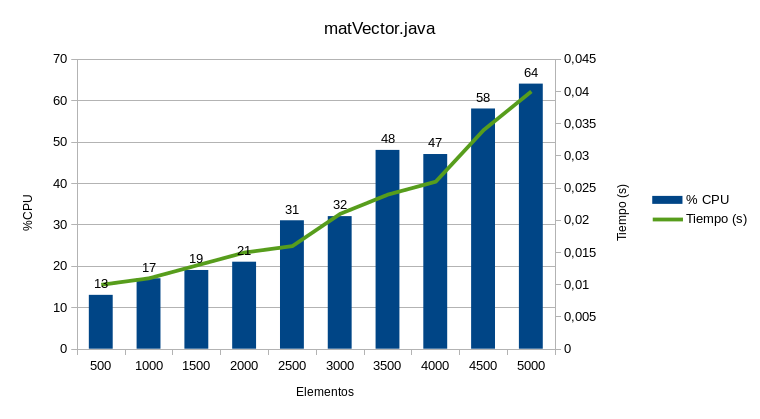
\includegraphics[scale=1]{matVector.png}
		\caption{Gráfica de matVector.}
		\label{fig: matVector}
	\end{center}
\end{figure}

\newpage
\section{\texttt{matVectorConcurrente.java}}
\noindent
Para las pruebas realizadas, hemos utilizado una matriz cuadrada con el mismo número de columnas que elementos tiene el vector por el cual se multiplica dicha matriz.
\begin{center}
	\begin{table}[htbp]
		\begin{center}
			\begin{tabular}{|c|c|c|}
				\hline
				\textbf{Elementos} & \textbf{\% CPU} & \textbf{Tiempo (s)}  \\
				\hline 
				$500$ & 25 & 0.019\\ \hline	
				$1000$ & 31 & 0.192\\ \hline
				$1500$ & 35 & 0.154\\ \hline
				$2000$ & 52 & 0.297\\ \hline
				$2500$ & 49 & 0.216\\ \hline
				$3000$ & 57 & 0.394\\ \hline
				$3500$ & 68 & 0.374\\ \hline
				$4000$ & 52 & 0.402\\ \hline
				$4500$ & 75 & 0.427\\ \hline
				$5000$ & 88 & 0.506\\ \hline				
				$10000$ & 100 & 0.906\\ \hline	
			\end{tabular}
			\caption{Valores de matVectorConcurrente.}
			\label{tabla:Valores de matVectorConcurrente}
		\end{center}
	\end{table}
\end{center}
\noindent
Con valores superiores a los de la tabla obtendremos un 100\% de uso de CPU y el tiempo irá aumentando hasta el punto en el que no entre en la memoria de la máquina virtual de java.
\begin{figure}
	\begin{center}
%		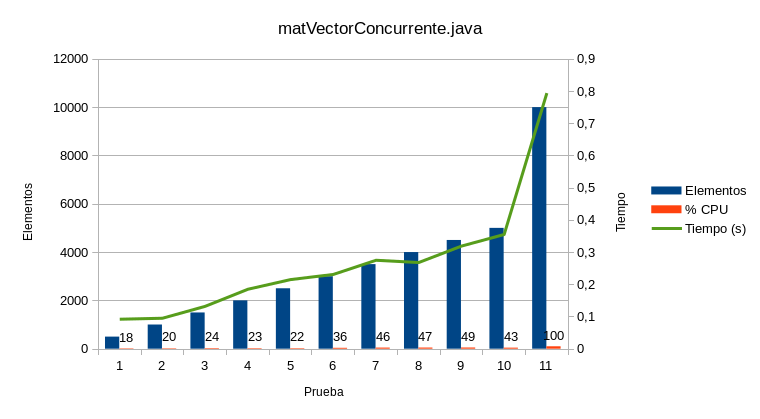
\includegraphics[scale=1]{matVectorConcurrente.png}
		\caption{Gráfica de matVectorConcurrente.}
		\label{fig: matVectorConcurrente}
	\end{center}	
\end{figure}


\newpage
\section{\texttt{prodMat.java}}
\noindent
Para las pruebas realizadas, hemos usado matrices cuadradas.
\begin{center}
	\begin{table}[htbp]
		\begin{center}
			\begin{tabular}{|c|c|c|}
				\hline
				\textbf{Elementos} & \textbf{\% CPU} & \textbf{Tiempo (s)}  \\
				\hline 
				$500$ & 19 & 0.282\\ \hline	
				$1000$ & 34 & 10.13\\ \hline
				$1500$ & 37 & 44.212\\ \hline
				$2000$ & 40 & 112.759\\ \hline
				$2500$ & 48 & 259.564\\ \hline
			\end{tabular}
			\caption{Valores de prodMat.}
			\label{tabla:Valores de prodMat}
		\end{center}
	\end{table}
\end{center}
\noindent
Viendo como va evolucionando la tabla, poner más valores es innecesario, ya que sería inviable para valores más altos.
\begin{figure}
	\begin{center}
%		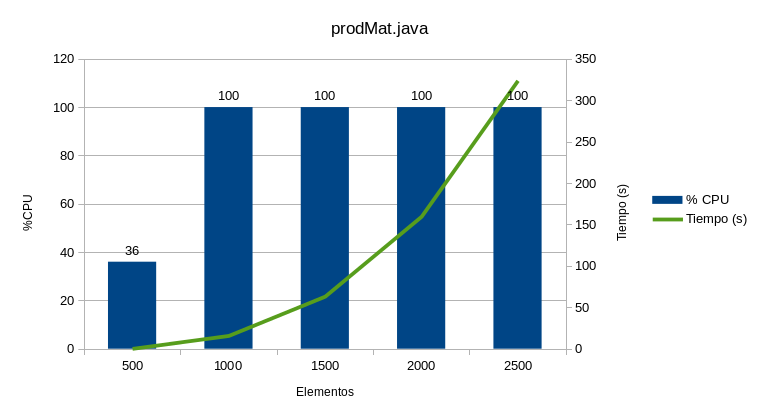
\includegraphics[scale=1]{prodMat.png}
		\caption{Gráfica de prodMat.}
		\label{fig: prodMat}
	\end{center}	
\end{figure}


\newpage
\section{\texttt{prodMatConcurrente.java}}
\noindent
Para las pruebas realizadas, hemos usado matrices cuadradas. Este algoritmo crea un hilo por cada elemento de la matriz resultante.
\begin{center}
	\begin{table}[htbp]
		\begin{center}
			\begin{tabular}{|c|c|c|}
				\hline
				\textbf{Elementos} & \textbf{\% CPU} & \textbf{Tiempo (s)}  \\
				\hline 
				$25$ & 33 & 0.052\\ \hline
				$50$ & 63 & 0.19\\ \hline
				$100$ & 99 & 0.839\\ \hline	
			\end{tabular}
			\caption{Valores de prodMatConcurrente.}
			\label{tabla:Valores de prodMatConcurrente}
		\end{center}
	\end{table}
\end{center}
\noindent
Debido al uso de excesivos hilos, si aumentamos el numero de filas/columnas a más de 100, el programa no ejecuta debido a que crea un hilo por elemento de la matriz resultante, por lo que satura la memoria de la máquina virtual de java.
\begin{figure}
	\begin{center}
%		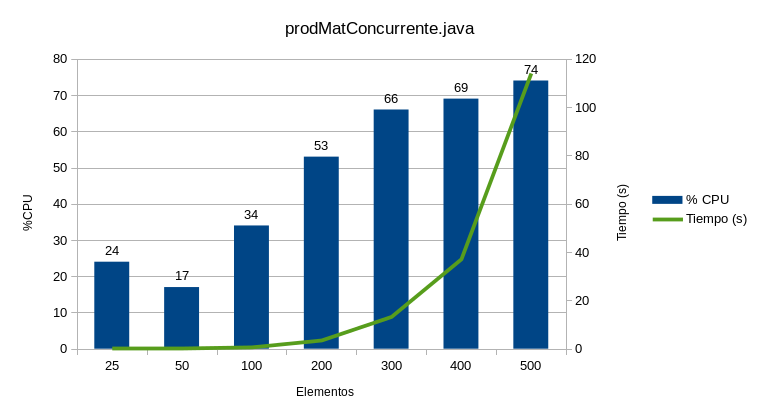
\includegraphics[scale=1]{prodMatConcurrente.png}
		\caption{prodMatConcurrente.}
		\label{fig: prodMatConcurrente}
	\end{center}	
\end{figure}


\newpage
\section{\texttt{prodMatAHiloPorFila.java}}
\noindent
Para las pruebas realizadas, hemos usado matrices cuadradas. Este algoritmo crea un hilo por cada fila de la matriz inicial, por lo que no genera tantísimos hilos como el algoritmo anterior.
\begin{center}
	\begin{table}[htbp]
		\begin{center}
			\begin{tabular}{|c|c|c|}
				\hline
				\textbf{Elementos} & \textbf{\% CPU} & \textbf{Tiempo (s)}  \\
				\hline 
				$500$ & 72 & 0.274\\ \hline	
				$1000$ & 88 & 1.756\\ \hline
				$1500$ & 81 & 5.172\\ \hline
				$2000$ & 92 & 12.37\\ \hline
				$2500$ & 98 & 25.733\\ \hline
				$3000$ & 100 & 49.419\\ \hline
				$3500$ & 84 & 105.38\\ \hline
				$4000$ & 94 & 191.47\\ \hline
				$4500$ & 100 & 344.6\\ \hline	
			\end{tabular}
			\caption{Valores de prodMatAHiloPorFila.}
			\label{tabla:Valores de prodMatAHiloPorFila}
		\end{center}
	\end{table}
\end{center}
\noindent
Si aumentamos el número de filas/columnas a mas de 4500, el programa tarda demasiado tiempo como para ser viable. Aún así, tarda mucho menos y no satura la memoria de la máquina virtual de java en comparación con su versión de hilo por elemento de la matriz resultante.
\begin{figure}
	\begin{center}
%		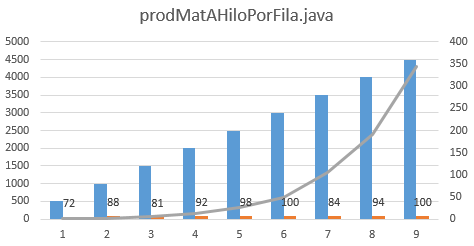
\includegraphics[scale=1]{prodMatAHiloPorFilaf.png}
		\caption{prodMatAHiloPorFila.}
		\label{fig: prodMatAHiloPorFila}
	\end{center}	
\end{figure}


\newpage
\section{Impresiones recabadas}
\noindent
Viendo los resultado obtenidos en las pruebas de los diversos algoritmos, podemos darnos cuenta de que el hecho de crear más hilos, no nos determina la velocidad con la que se ejecutará un programa.\\
Esto es así, debido a que la creación de hilos, nos genera un coste en tiempo y en memoria que puede ser crucial en otros aspectos.\\
El caso más evidente donde podemos contrastar lo descrito en este apartado lo tenemos a simple vista en los algoritmos \texttt{prodMatConcurrente.java} (donde creamos un hilo por elemento de la matriz resultante) y \texttt{prodMatAHiloPorFila.java} (donde creamos un hilo por fila de la primera matriz). En estos algoritmos que, hacen exáctamente lo mismo, podemos ver que tener un mayor número de hilos, no nos asegura una mayor velocidad ya que, aparte de la velocidad, la memoria, es un elemento a tener muy en cuenta, ya que en el primero se satura con algo más de 100 elementos, mientras que el segundo acepta más de 4500 y no da problemas respecto a la memoria.

\end{document}